\documentclass[11pt]{article}
\usepackage{geometry}                % See geometry.pdf to learn the layout options. There are lots.
\geometry{letterpaper}                   % ... or a4paper or a5paper or ... 
%\geometry{landscape}                % Activate for for rotated page geometry
%\usepackage[parfill]{parskip}    % Activate to begin paragraphs with an empty line rather than an indent
\usepackage{graphicx}
\usepackage{amssymb}
\usepackage{amsmath}
\usepackage{epstopdf}
\usepackage{hyperref}
\DeclareGraphicsRule{.tif}{png}{.png}{`convert #1 `dirname #1`/`basename #1 .tif`.png}



\graphicspath{
{/Users/Andy/Cruises_Research/Analysis/Andy_Pickering/tiwe_patch_gamma/figures/}
}

\title{Patch/Gamma Analysis for TIWEchameleon patches}
\author{Andy Pickering}
%\date{}                                           % Activate to display a given date or no date



\begin{document}
\maketitle

\tableofcontents
\newpage

%~~~~~~~~~~~~~~~~~~~~~
\section{Overview}

The goal of this analysis is to compute mixing efficency ($\Gamma$) for patches in TIWE chameleon profiles, and see if we obtain values close to $\Gamma=0.2$.

%~~~~~~~~~~~~~~~~~~~~~
\section{Data}

Data are made by the `Chameleon' microstructure profiler near the equator during the `TIWE' experiment. Data was shared by JN and my local copy is at: \newline \verb+/Users/Andy/Dropbox/AP_Share_With_JN/date_from_jim/Tiwe91+

\medskip

I'm using the raw Chameleon data files in: \newline
\verb+/Users/Andy/Dropbox/AP_Share_With_JN/date_from_jim/Tiwe91/cham/tw/+

\medskip

All my analysis is in the main folder: \newline  \verb+/Users/Andy/Cruises_Research/ChiPod/TIWE+


%~~~~~~~~~~~~~~~~~~~~~
\section{Methods}

\begin{itemize}

\item \verb+Process_tiwe_rawprofiles_AP.m+  Processes raw Chameleon files and saves `cal2' files which have the raw/ high-res profiles of temp and salinity. These are used to identify patches.

\item \verb+FindPatches_tiwe_Raw.m+ Identifies patches in the profiles made by \verb+Process_tiwe_rawprofiles_AP.m+, using potential temperature.

\item \verb+Run_tiwe_AP_forPatches.m+ Runs the Chameleon processing (including $\chi$ and $\epsilon$) for just the patches identified in \verb+FindPatches_tiwe_Raw.m+ .

\item \verb+Run_tiwe_AP.m+ Runs the standard Chameleon processing, producing 1m avg quantities.

\item \verb+Combine_tiwe_avg_profiles.m+ Combines the avg profiles made in \verb+Run_tiwe_AP.m+ into a single structure with common depths.

\item \verb+Compute_N2_dTdz_patches_tiwe.m+ Computes $N^2$ and $T_z$ for patches, using several different methods.

\end{itemize}

\medskip

%%~~~~~~~
%\subsection{Overturns}
%Overturns (patches) are detected for each profile, using potential temperature.

%~~~~~~~
\subsection{dTdz}

Temperature gradient is computed for each patch using the following methods:
\begin{enumerate}
\item dtdz1 : Take the range of T over the patch and divided by patch height
\item dtdz2 : Fit a straight line to sorted T using \verb+polyfit+
\item dtdz3 : Use the 'bulk gradient' from Smyth et al 2001, which is the rms fluctuation from the background (sorted) temperature, divided by the thorpe scale (the rms re-ordering distances).
\end{enumerate}


%~~~~~~~
\subsection{N2}

$N^2$ is computed for each patch using the following methods:
\begin{enumerate}
\item $N^2_1$ : Take the range of potential density over the patch divided by the patch height ($d\rho/dz$), then compute $N^2=\frac{-g}{\rho_o}\frac{d\rho}{dz}$ where $\rho_o$ is the mean potential density over the patch.
\item $N^2_2$ : Fit a straight line to sorted potential density using polyfit to get $d\rho/dz$, then compute N2.
\item $N^2_3$ : Use 'bulk gradient' . This is calculated from the bulk $T_z$, using a linear fit between density and temperature.
\item $N^2_4$ : Compute $N^2$ from the sorted profile (sorted by potential density) using \verb+sw_bfreq+, then take average over the patch. I believe this method is used by some commonly-used overturn codes.
\end{enumerate}


%~~~~~~~
\subsection{Mixing Efficiency}

Mixing Efficiency $\Gamma$ is computed from the following equation using differerent $N^2$ and $dT/dz$ values.
\begin{equation}
\Gamma=\frac{N^2 \chi}{2\epsilon T_{z}^{2}} 
\end{equation}
$\chi$ and $\epsilon$ are computed over each patch from the Chameleon data. Gamma is computed for the following 4 combinations:
\begin{enumerate}
\item  $N^2_1$, dtdz1
\item $N^2_2$, dtdz2
\item $N^2_3$, dtdz3
\item $N^2_4$, dtdz2
\end{enumerate}
Values where $\epsilon$ is below the noise floor of $log_{10}[\epsilon]=-8.5$ are discarded (using these values does have a significant impact on the mean/median of the resulting distribution).



%~~~~~~~~~~~~~~~~~~~~~
\section{Results}

\begin{itemize}
\item For some reason many $\chi$ values below 150db are bad/missing? Not sure why.
\item The median $\Gamma$ computed using the 1m avg data is $0.063$ (Figure \ref{avggam})}.
\item Gamma computed over patches w/ linear fits is slightly higher than the binned gamma, but still less than $0.2$ (Figure \ref{patchgam}).
\end{itemize}
%

\begin{figure}[htbp]
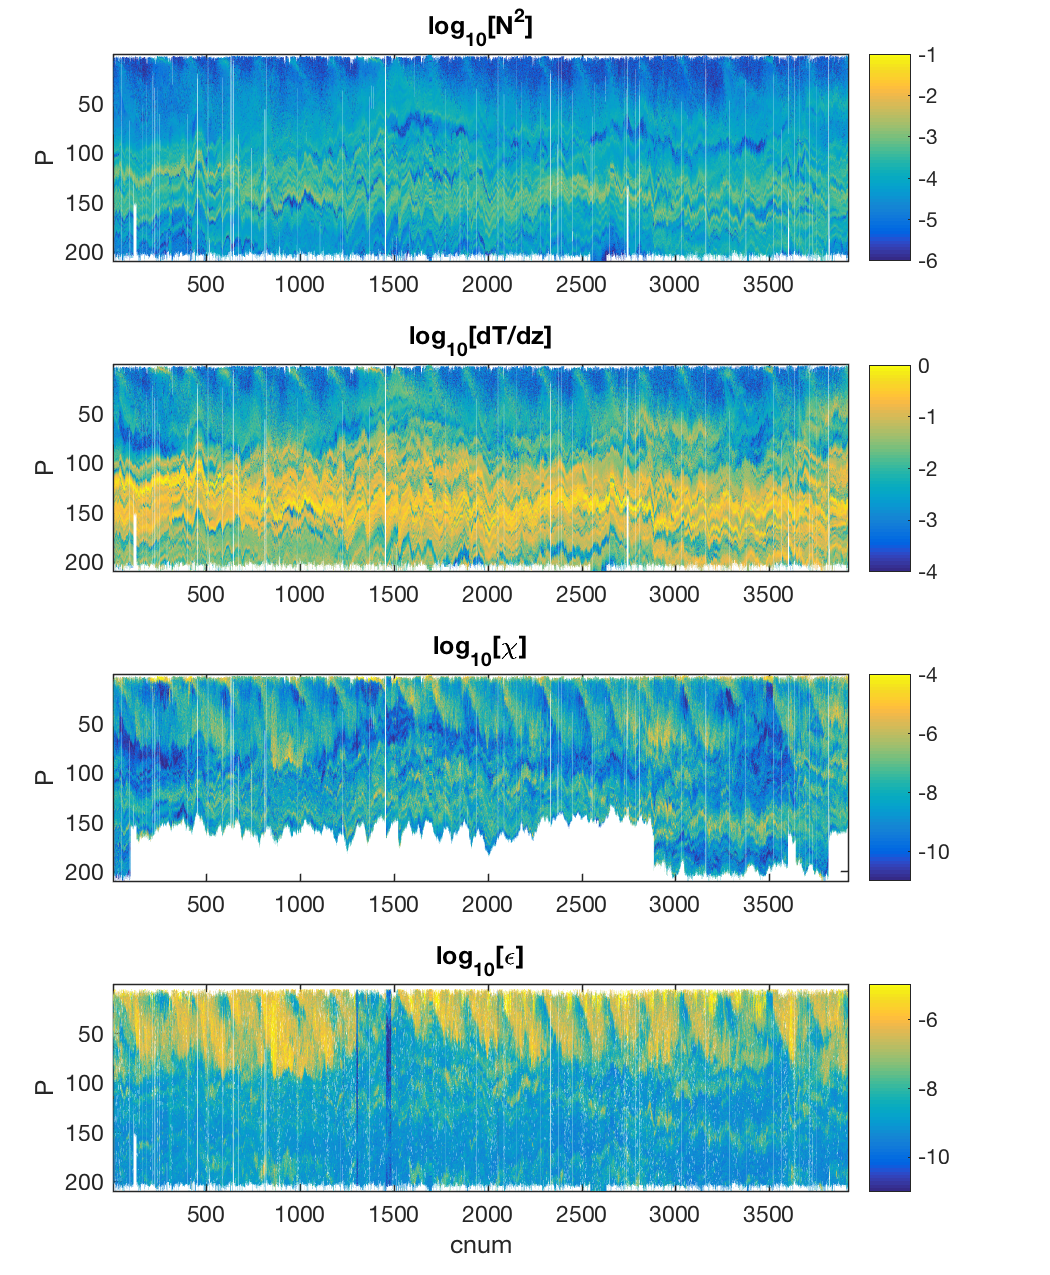
\includegraphics[scale=0.8]{tiwe_avgCombine_N2_dtdz_chi_eps.png}
\caption{Pcolor of the combined 1m avg chameleon data for TIWE. * Note for some reason many $\chi$ values below 150db are bad/missing.}
\label{}
\end{figure}

\begin{figure}[htbp]
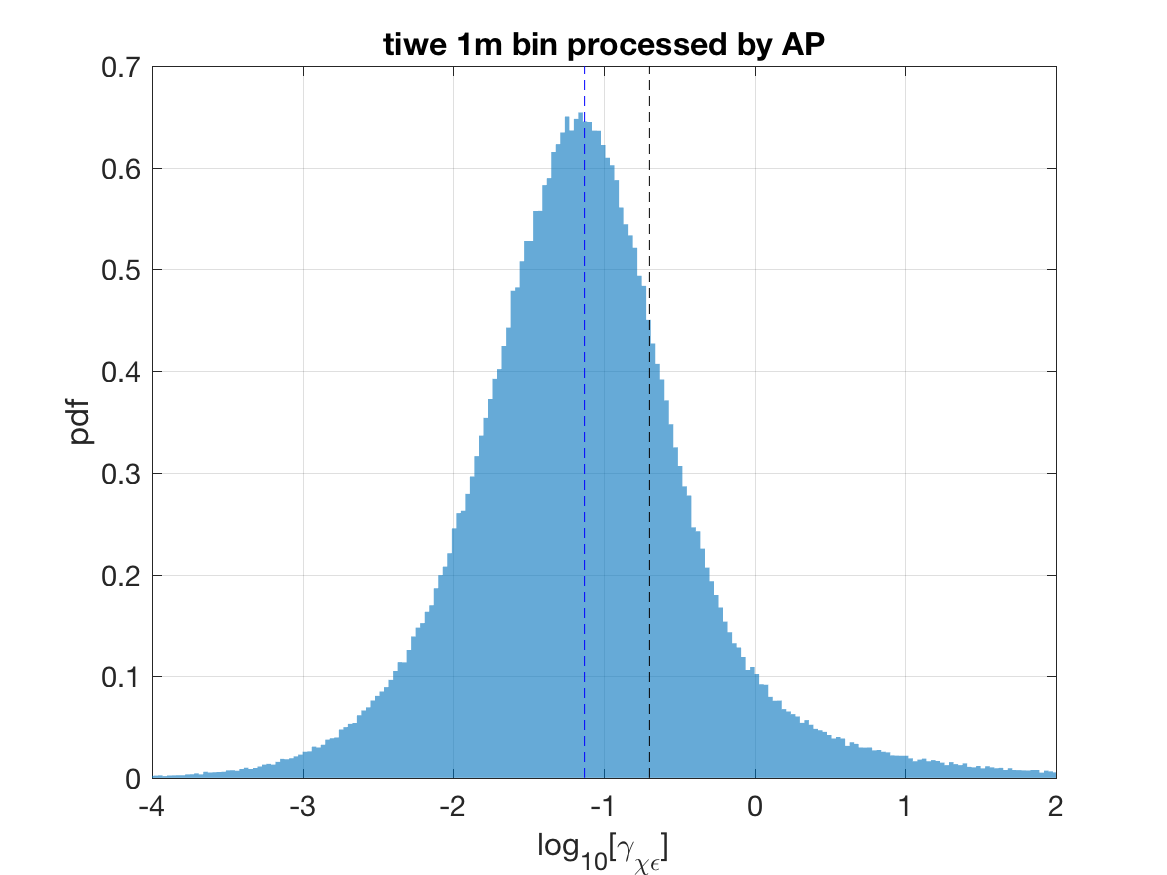
\includegraphics[scale=0.8]{tiwe_avgCombine_gamma.png}
\caption{Histogram of $\Gamma$ for 1m avg chameleon profiles. Vertical dashed line shows $\Gamma=0.2$.}
\label{avggam}
\end{figure}
%


\begin{figure}[htbp]
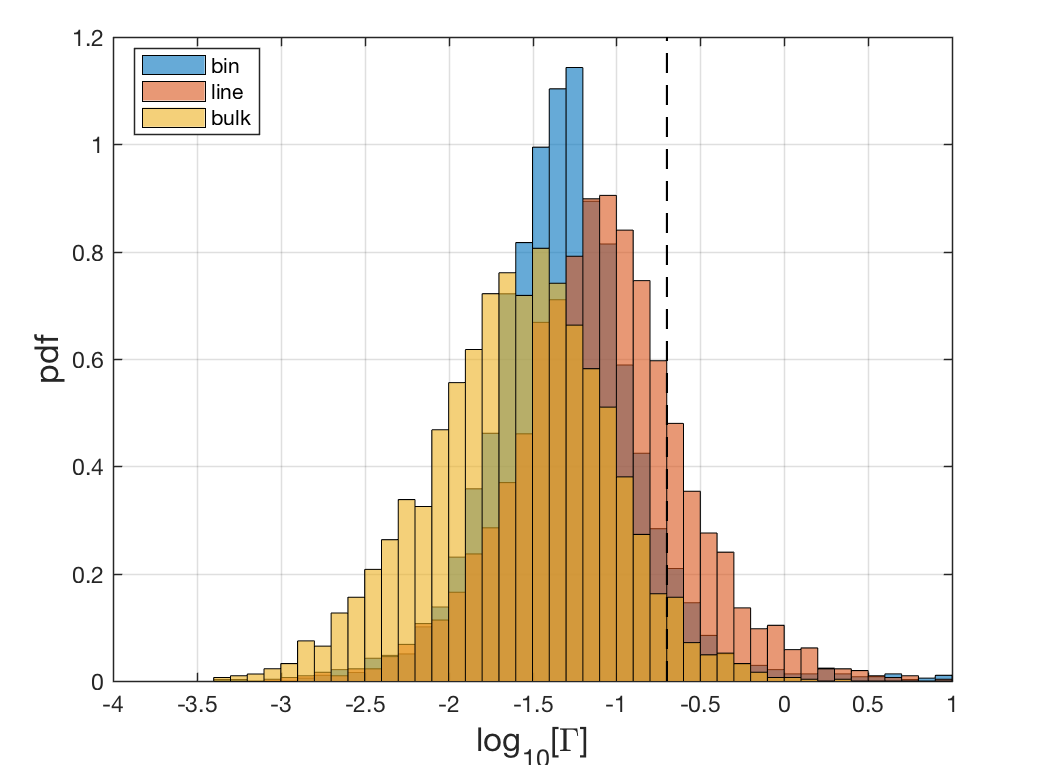
\includegraphics[scale=0.8]{tiwe_minOT_25_usetemp_1_gammas_hist.png}
\caption{Histogram of $\Gamma$ for patches, using different estimates of $N^2$ and $T_z$. Vertical dashed line shows $\Gamma=0.2$.}
\label{patchgam}
\end{figure}
%





\clearpage
%~~~~~~~~~~~~~~~~~~~~~
\section{Comparison to previous analysis}

Bill send me results of a previous patch analysis for tiwe: \verb+events_TIWE.mat+ . Here i'll compare my results to those. See \verb+compare_patches_tiwe_AP_Bill.m+ . It looks like my values of $N^2$, $T_z$, and $\chi$ tend to be smaller than Bill's (Figure \ref{comp_bill_ap_1}). Gamma computed from my patch values is smaller than 0.2, centered around..., while gamma from Bill's values is larger than 0.2, centered at about .

**Note that the number of patches I found is much larger than those in Bill's data. I'm not sure if this is because he joined some patches, or only looked at certain profiles, or had some other threshold? His data doesn't give info on patch locations or profiles so I can't compare them directly to mine.

\begin{figure}[htbp]
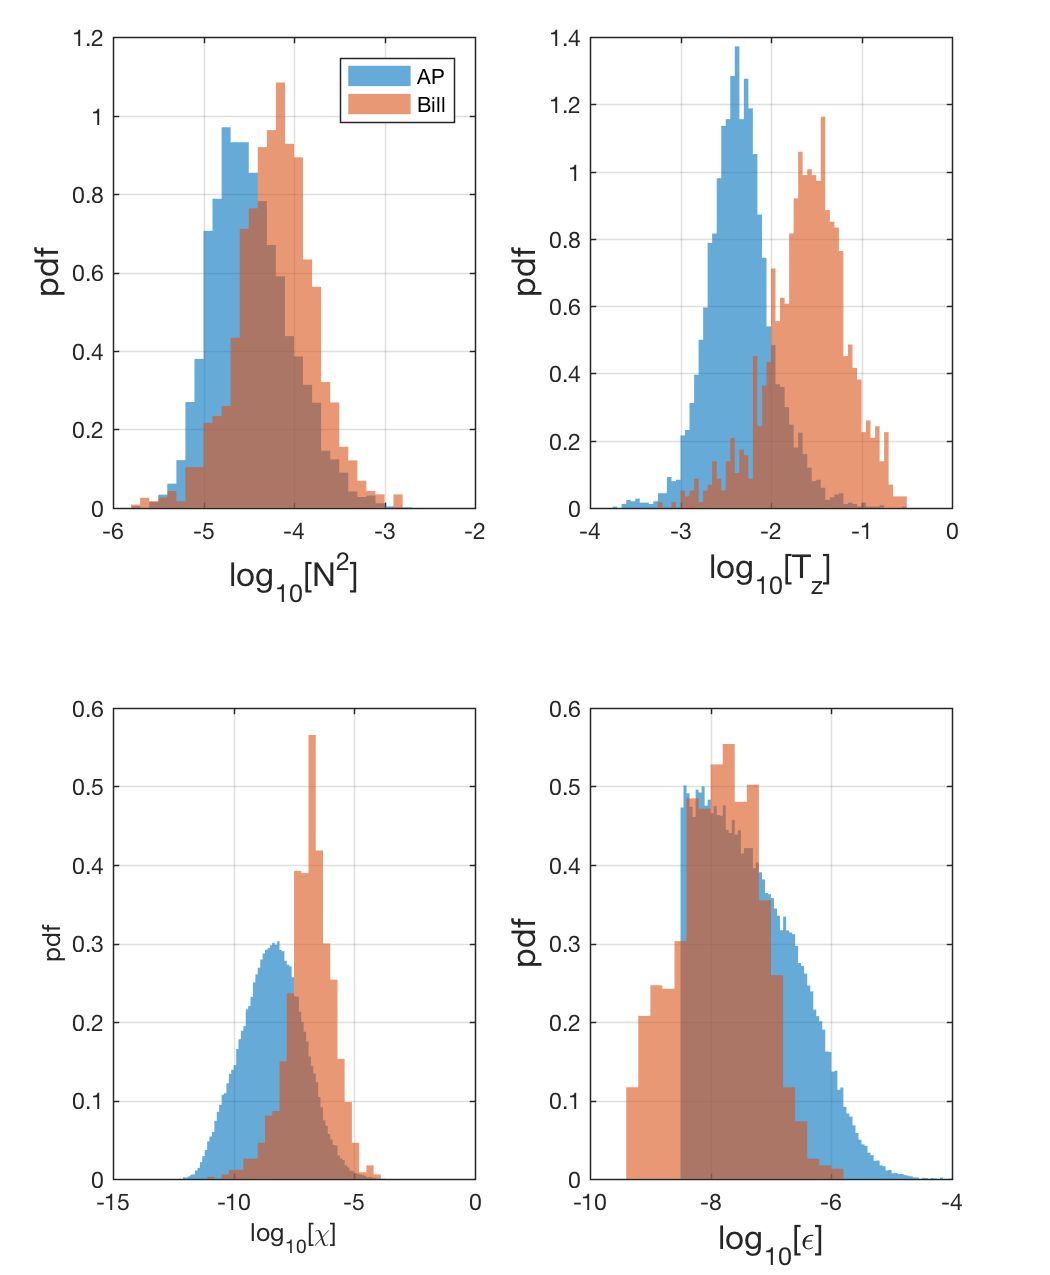
\includegraphics[scale=0.8]{tiwe_minOT_15_usetemp_1_n2_tz_chi_eps_apvsbill_hist.png}
\caption{Histograms of $N^2$ , $T_z$, $\chi$, and $\epsilon$ for patches analyzed by myself and Bill.}
\label{comp_bill_ap_1}
\end{figure}
%




%
%%~~~~~~~~~~~~~~~~~~~~~
%\section{Comparison to binned $\Gamma$}
%
%The mixing efficiencies computed by patch are compared to values computed using the binned (1m) chameleon data. I found the closest binned data point to each patch and computed gamma with those values. Using the binned data to compute $\Gamma$ results in lower values of mixing efficiencies by about a factor of 2 (Figure \ref{gam_binVspatch}).
%
%\begin{figure}[htbp]
%\includegraphics[scale=0.8]{eq14_cham_gamma_binVspatch.png}
%\caption{$\Gamma$ computed from binned data (at patch locations) and for patches. Vertical lines indicate medians.}
%\label{gam_binVspatch}
%\end{figure}
%
%\begin{figure}[htbp]
%\includegraphics[scale=0.8]{eq14_cham_LOGgamma_binVspatch.png}
%\caption{$\Gamma$ computed from binned data (at patch locations) and for patches. Vertical lines indicate medians. Black dashed line is log10[0.2].}
%\label{LOGgam_binVspatch}
%\end{figure}
%
%
%\begin{figure}[htbp]
%\includegraphics[scale=0.8]{eq14_binVspatch_gamma.png}
%\caption{$log_{10}\Gamma$ computed from binned data (at patch locations) vs for patches. Red lines indicate $\Gamma=0.2$. Diagonal black line is slope of 1.}
%\label{}
%\end{figure}
%
%
%\begin{figure}[htbp]
%\includegraphics[scale=0.8]{eq14_cham_gamma_binVspatch_scatter.png}
%\caption{Scatter plot of $\Gamma$ computed from binned data (at patch locations) and for patches.}
%\label{gam_binVspatch_scat}
%\end{figure}

%
%
%
%%~~~~~~~~~~~~~~~~~~~~~
%\section{Comparison of binned profiles to patch values}
%
%\begin{figure}[htbp]
%\includegraphics[scale=0.8]{eq14_binVspatch_N2dTdzChiEps.png}
%\caption{2D histograms of binned vs patch data (at patch locations) .}
%\label{binVspatch_2d}
%\end{figure}
%
%
%\begin{figure}[htbp]
%\includegraphics[scale=0.8]{eq14_cham_gamma_binVspatch_hists.png}
%\caption{Histograms of binned data (at patch locations) and patche data.}
%\label{binVspatch_hists}
%\end{figure}
%





\end{document}  


